\documentclass[11pt,a4paper]{article}

\usepackage[utf8]{inputenc}
\usepackage[T1]{fontenc}
\usepackage[brazil]{babel}
\usepackage{lmodern}
\usepackage[margin=2.5cm]{geometry}
\usepackage{amsmath,amssymb}
\usepackage{graphicx}
\usepackage{booktabs}
\usepackage{multirow}
\usepackage{float}
\usepackage[font=small,labelfont=bf]{caption}
\usepackage[table]{xcolor}
\usepackage{hyperref}

\hypersetup{colorlinks=true, linkcolor=blue!50!black, urlcolor=blue!50!black, citecolor=blue!50!black}
\graphicspath{{./}}
\newcommand{\bom}[1]{\textbf{#1}}
\newcommand{\ruim}[1]{\textcolor{red!70!black}{#1}}

\title{Block Influence e poda de camadas no GraphPFN}
\author{Isabelly Pinheiro}
\date{Outubro de 2026}

\begin{document}
\maketitle

\begin{abstract}
Avaliamos se é possível remover camadas inteiras do GraphPFN, sem re-treino, escolhendo-as pela métrica de \emph{Block Influence} (BI). O modelo completo foi avaliado com o pipeline oficial e splits oficiais em cinco datasets (classificação binária, multiclasse e regressão), com três sementes. O BI escolhe camadas melhor que o acaso: removendo 3 camadas, a ordem por BI retém 70\% do desempenho, contra 24\% de uma ordem aleatória. Mesmo assim, nenhuma estratégia mantém 95\% do desempenho com mais de uma camada removida. Remover 5 camadas leva a maioria dos datasets ao nível do acaso. A causa principal é que o BI calculado como média sobre todos os tokens marca como pouco importantes justamente as camadas 0 e 1, que são as mais importantes para a predição. Calcular o BI apenas no token usado na predição (token-alvo) corrige parte do problema, mas não o suficiente para tornar a poda viável além de uma camada.
\end{abstract}

\tableofcontents

%==============================================================================
\section{Objetivo}
%==============================================================================

A pergunta central é: \textbf{dá para remover camadas do GraphPFN escolhidas por Block Influence sem perder desempenho?}

Para que a poda seja considerada válida, exigimos quatro critérios:

\begin{table}[H]
\centering
\caption{Critérios de validade da poda.}
\label{tab:criterios}
\begin{tabular}{@{}clp{7.2cm}@{}}
\toprule
& Critério & Como é testado \\
\midrule
V1 & Baseline funciona & Modelo completo bem acima do acaso, com pipeline e splits oficiais \\
V2 & Poda retém desempenho & Desempenho retido $\geq 95\%$ após remover camadas \\
V3 & BI é melhor que o acaso & Ordem por BI comparada a 5 ordens aleatórias \\
V4 & BI reflete importância real & Correlação de Spearman entre BI e a queda ao remover cada camada sozinha \\
\bottomrule
\end{tabular}
\end{table}

%==============================================================================
\section{O modelo}
%==============================================================================

O GraphPFN é o modelo tabular \textbf{LimiX-16M}, um \emph{prior-data fitted network} (PFN), com \textbf{adaptadores de grafo} inseridos após cada uma das suas 12 camadas. O modelo faz aprendizado em contexto: não é treinado no dataset avaliado. Os nós de treino, com rótulo, entram como contexto e o modelo infere os rótulos dos nós de teste em um único \emph{forward}.

Cada camada (\texttt{GraphPFNLayerWrapper}) executa, em sequência:
\begin{enumerate}
  \item \textbf{Bloco LimiX} (\texttt{EncoderBaseLayer}, arquitetura \texttt{fmfmsm}): atenção entre features $\to$ MLP $\to$ atenção entre features $\to$ MLP $\to$ atenção entre amostras (nós de teste olham apenas os de treino) $\to$ MLP;
  \item \textbf{Atenção de grafo}: $h \leftarrow h + \mathrm{GraphAttention}(\mathrm{LayerNorm}(h))$, troca de mensagens pelas arestas;
  \item \textbf{MLP de grafo}: $h \leftarrow h + \mathrm{MLP}(\mathrm{LayerNorm}(h))$.
\end{enumerate}

\paragraph{Tokens.} Cada nó vira $G+1$ tokens de dimensão 192: $G = \lceil (F+8)/2 \rceil$ tokens de grupos de features (as $F$ features mais 8 aleatórias, agrupadas de 2 em 2) e \textbf{1 token-alvo}, que carrega o rótulo nos nós de treino e fica mascarado nos de teste. \textbf{A predição sai apenas do token-alvo dos nós de teste.} No cora, por exemplo, o estado interno tem forma $1 \times 2708 \times 37 \times 192$: são 36 tokens de feature para cada token-alvo.

\begin{table}[H]
\centering
\caption{Parâmetros por componente.}
\label{tab:params}
\begin{tabular}{@{}lrr@{}}
\toprule
Componente & Parâmetros & \% da camada \\
\midrule
Bloco LimiX (atenções + 3 MLPs) & 1\,327\,104 & 81,7 \\
Adaptador de grafo: atenção & 148\,608 & 9,2 \\
Adaptador de grafo: MLP & 148\,416 & 9,1 \\
\midrule
Total por camada & 1\,624\,128 & 100,0 \\
\midrule
\multicolumn{3}{@{}l}{Modelo inteiro: 20,09\,M parâmetros; as 12 camadas somam 19,49\,M (97,0\%).} \\
\multicolumn{3}{@{}l}{Remover uma camada reduz 8,08\% dos parâmetros.} \\
\bottomrule
\end{tabular}
\end{table}

%==============================================================================
\section{Metodologia}
%==============================================================================

\subsection{Datasets e pipeline}

Todos os experimentos usam o \textbf{grafo completo} e os \textbf{splits oficiais}. O pré-processamento é o mesmo de \texttt{graphpfn.inference.icl.predict\_icl}:
\begin{itemize}
  \item grafo: remoção de self-loops, remoção de arestas duplicadas e simetrização (\texttt{prepare\_graph});
  \item features: \texttt{prepare\_features\_tensor}, com PCA para 64 dimensões em cora e pubmed (valor recomendado pelo README do GraphPFN para features de alta dimensão);
  \item regressão: alvo padronizado (\texttt{standardize\_targets}) e desnormalizado na saída;
  \item inferência em \texttt{bfloat16}, como no pipeline oficial; 1 membro de ensemble.
\end{itemize}

\begin{table}[H]
\centering
\caption{Datasets avaliados.}
\label{tab:datasets}
\begin{tabular}{@{}llrrl@{}}
\toprule
Dataset & Tarefa & Nós & Nós de contexto (treino) & Métrica \\
\midrule
tolokers-2   & Classificação binária & 11\,758 & 1\,175 & ROC-AUC \\
cora         & Multiclasse (7)       & 2\,708  & 140    & Acurácia \\
pubmed       & Multiclasse (3)       & 19\,717 & 60     & Acurácia \\
city-roads-M & Regressão             & 57\,073 & 3\,610 & $R^2$ \\
artnet-views & Regressão             & 50\,405 & 5\,040 & $R^2$ \\
\bottomrule
\end{tabular}
\end{table}

Cada experimento é repetido com as sementes 0, 1 e 2. A semente fixa as features aleatórias e o \emph{positional embedding} do LimiX, de modo que modelo completo e modelo podado são comparados com a mesma semente.

\subsection{Desempenho retido}

Para comparar tarefas com métricas diferentes, normalizamos o desempenho pelo nível do acaso:
\begin{equation}
\text{retido}(\%) = 100 \cdot \frac{s_{\text{podado}} - s_{\text{acaso}}}{s_{\text{completo}} - s_{\text{acaso}}},
\end{equation}
onde $s_{\text{acaso}}$ é 0,5 para ROC-AUC, a frequência da classe majoritária no teste para acurácia e 0 para $R^2$. 100\% significa igual ao modelo completo; 0\% significa igual a chutar; valores negativos significam pior que o acaso.

\subsection{Block Influence}

Para cada camada $\ell$, comparamos o estado de entrada $h_\ell^{in}$ e o de saída $h_\ell^{out}$ token a token:
\begin{equation}
BI_{\cos}(\ell) = 1 - \cos\!\left(h_\ell^{in}, h_\ell^{out}\right), \qquad
BI_{\text{ang}}(\ell) = \frac{\arccos\!\left(\cos(h_\ell^{in}, h_\ell^{out})\right)}{\pi}.
\end{equation}
BI baixo indica que a camada altera pouco o estado e, segundo a hipótese do ShortGPT, poderia ser removida. Calculamos o BI de duas formas:
\begin{itemize}
  \item \textbf{BI de todos os tokens}: média sobre os $N \times (G+1)$ tokens. É a forma usual.
  \item \textbf{BI do token-alvo}: média apenas sobre os tokens-alvo dos nós de teste, que são os únicos que o decodificador lê.
\end{itemize}
A distinção importa porque, na média sobre todos os tokens, os tokens de feature (por exemplo, 36 de cada 37 no cora) dominam, enquanto a predição depende só do token-alvo. O BI também foi calculado separadamente para cada sub-bloco (LimiX, atenção de grafo, MLP de grafo).

\subsection{Estratégias de poda}

Para cada dataset, as camadas são ordenadas e removidas cumulativamente: com $k$ camadas removidas, saem as $k$ primeiras da ordem, para $k = 1, \dots, 11$. A remoção é feita retirando a camada da lista \texttt{transformer\_encoder.layers}; a saída da camada anterior passa direto para a seguinte.

\begin{itemize}
  \item \textbf{BI de todos os tokens}: menor BI sai primeiro;
  \item \textbf{BI do token-alvo}: menor BI sai primeiro;
  \item \textbf{Ablação individual (val)}: sai primeiro a camada cuja remoção isolada causa a menor queda na \emph{validação}. Usa rótulos e serve como referência do que seria uma ordem quase ótima;
  \item \textbf{Aleatória}: 5 permutações fixas (controle do critério V3).
\end{itemize}

%==============================================================================
\section{Resultados}
%==============================================================================

\subsection{V1: o modelo completo funciona}

\begin{table}[H]
\centering
\caption{Desempenho do modelo completo no teste (média $\pm$ desvio-padrão em 3 sementes).}
\label{tab:baseline}
\begin{tabular}{@{}llccc@{}}
\toprule
Dataset & Métrica & Modelo completo & Acaso & Validação \\
\midrule
tolokers-2   & ROC-AUC  & \bom{0,860} $\pm$ 0,001 & 0,500 & 0,852 \\
cora         & Acurácia & \bom{0,674} $\pm$ 0,006 & 0,319 & 0,673 \\
pubmed       & Acurácia & \bom{0,714} $\pm$ 0,010 & 0,413 & 0,727 \\
city-roads-M & $R^2$    & \bom{0,640} $\pm$ 0,001 & 0     & 0,647 \\
artnet-views & $R^2$    & \bom{0,621} $\pm$ 0,000 & 0     & 0,618 \\
\bottomrule
\end{tabular}
\end{table}

O modelo completo fica bem acima do acaso em todos os datasets e varia muito pouco entre sementes. \textbf{V1 é atendido}, e esses valores são a referência (100\%) de todas as comparações de poda.

\subsection{Block Influence por camada}

\begin{table}[H]
\centering
\caption{BI (cosseno) por camada inteira, média de 3 sementes. Em negrito, as 5 camadas de menor BI de cada linha, isto é, as primeiras a serem removidas.}
\label{tab:bi}
\setlength{\tabcolsep}{3.6pt}
\small
\begin{tabular}{@{}l*{12}{c}@{}}
\toprule
Dataset & L0 & L1 & L2 & L3 & L4 & L5 & L6 & L7 & L8 & L9 & L10 & L11 \\
\midrule
\multicolumn{13}{@{}l}{\emph{BI de todos os tokens}} \\
tolokers-2   & ,170 & \bom{,047} & \bom{,051} & \bom{,113} & \bom{,097} & ,260 & ,326 & ,211 & ,321 & ,446 & \bom{,164} & ,447 \\
cora         & \bom{,133} & \bom{,027} & \bom{,061} & \bom{,154} & \bom{,100} & ,255 & ,324 & ,210 & ,328 & ,458 & ,242 & ,519 \\
pubmed       & \bom{,131} & \bom{,030} & \bom{,062} & \bom{,160} & \bom{,100} & ,252 & ,317 & ,222 & ,345 & ,441 & ,243 & ,499 \\
city-roads-M & \bom{,179} & \bom{,019} & \bom{,047} & \bom{,102} & \bom{,121} & ,271 & ,324 & ,234 & ,328 & ,478 & ,244 & ,546 \\
artnet-views & \bom{,127} & \bom{,013} & \bom{,047} & \bom{,104} & \bom{,106} & ,282 & ,350 & ,223 & ,359 & ,456 & ,236 & ,587 \\
\midrule
\multicolumn{13}{@{}l}{\emph{BI do token-alvo}} \\
tolokers-2   & ,858 & ,488 & \bom{,016} & \bom{,023} & \bom{,063} & ,158 & ,256 & \bom{,139} & ,190 & ,229 & \bom{,072} & ,182 \\
cora         & ,740 & ,525 & \bom{,014} & \bom{,024} & \bom{,057} & ,151 & ,229 & \bom{,141} & ,167 & ,226 & \bom{,071} & ,285 \\
pubmed       & ,753 & ,543 & \bom{,015} & \bom{,026} & \bom{,054} & ,151 & ,215 & \bom{,146} & ,161 & ,209 & \bom{,078} & ,194 \\
city-roads-M & ,727 & \bom{,046} & \bom{,014} & \bom{,022} & \bom{,065} & ,182 & ,234 & ,143 & ,182 & ,226 & \bom{,078} & ,288 \\
artnet-views & ,713 & \bom{,029} & \bom{,015} & \bom{,022} & \bom{,062} & ,191 & ,242 & ,149 & ,187 & ,212 & \bom{,071} & ,293 \\
\bottomrule
\end{tabular}
\end{table}

\begin{figure}[H]
\centering
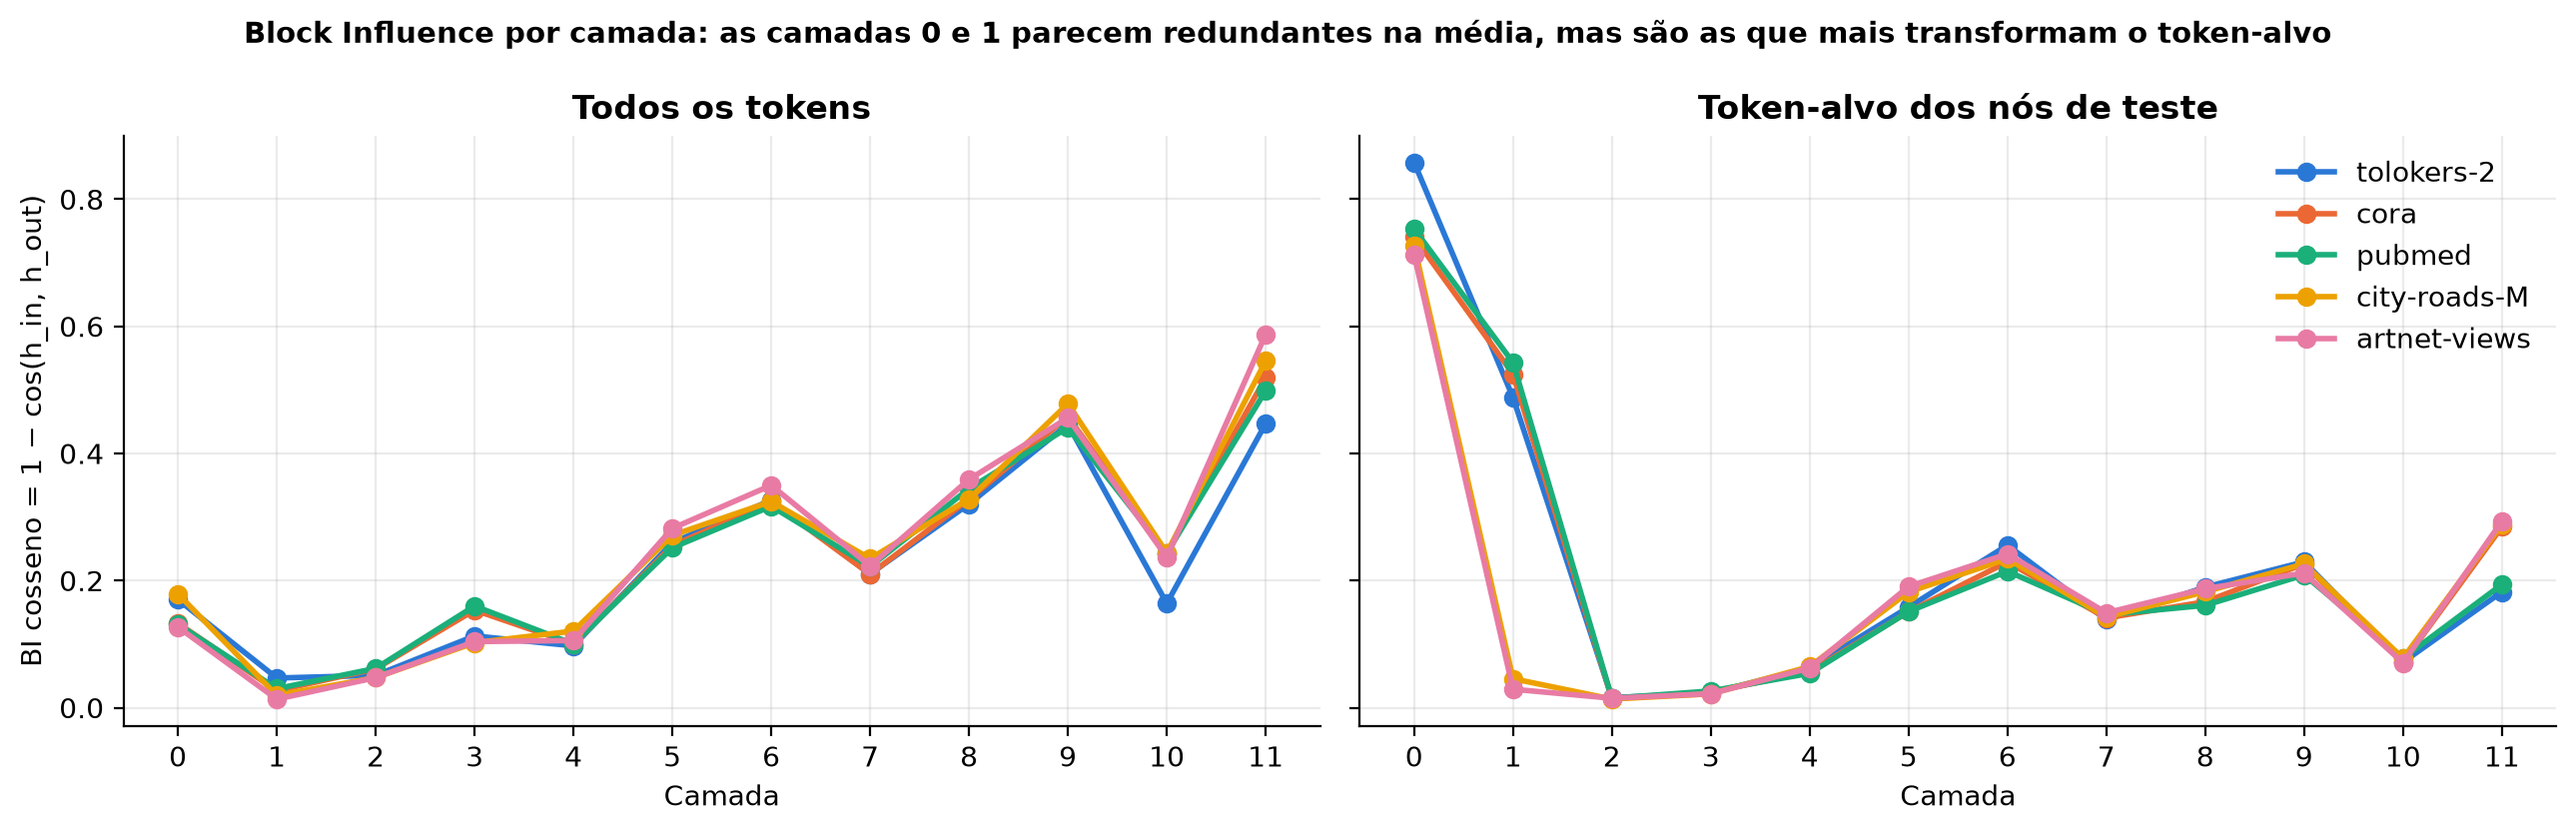
\includegraphics[width=\textwidth]{bi_por_camada.png}
\caption{BI por camada em cada dataset.}
\label{fig:bi}
\end{figure}

Principais observações:
\begin{itemize}
  \item \textbf{O BI é estável.} O desvio-padrão entre sementes é no máximo 0,0034. O ranking de BI é praticamente o mesmo em todos os datasets (Spearman entre 0,96 e 1,00), e cosseno e angular dão o mesmo ranking (Spearman $\geq 0{,}99$). A escolha entre cosseno e angular não muda nada; por isso o resto do relatório usa apenas o cosseno.
  \item \textbf{As duas formas de BI discordam nas camadas 0 e 1.} Na média de todos os tokens, as camadas 0 e 1 estão entre as de menor BI. No token-alvo, a camada 0 é a que mais muda o estado (0,71 a 0,86) em todos os datasets, e a camada 1 também muda muito na classificação ($\approx 0{,}5$), mas pouco na regressão ($\approx 0{,}03$). É nessas camadas que a informação das features e do contexto rotulado chega ao token que é decodificado.
  \item \textbf{Quase toda a transformação vem do bloco LimiX.} Os adaptadores de grafo alteram muito pouco o estado: BI de 0,001 a 0,09 na atenção de grafo e de 0,001 a 0,05 no MLP de grafo, com exceção do MLP de grafo da camada 11 (0,15). Veja a Figura~\ref{fig:subbloco}.
\end{itemize}

\begin{figure}[H]
\centering
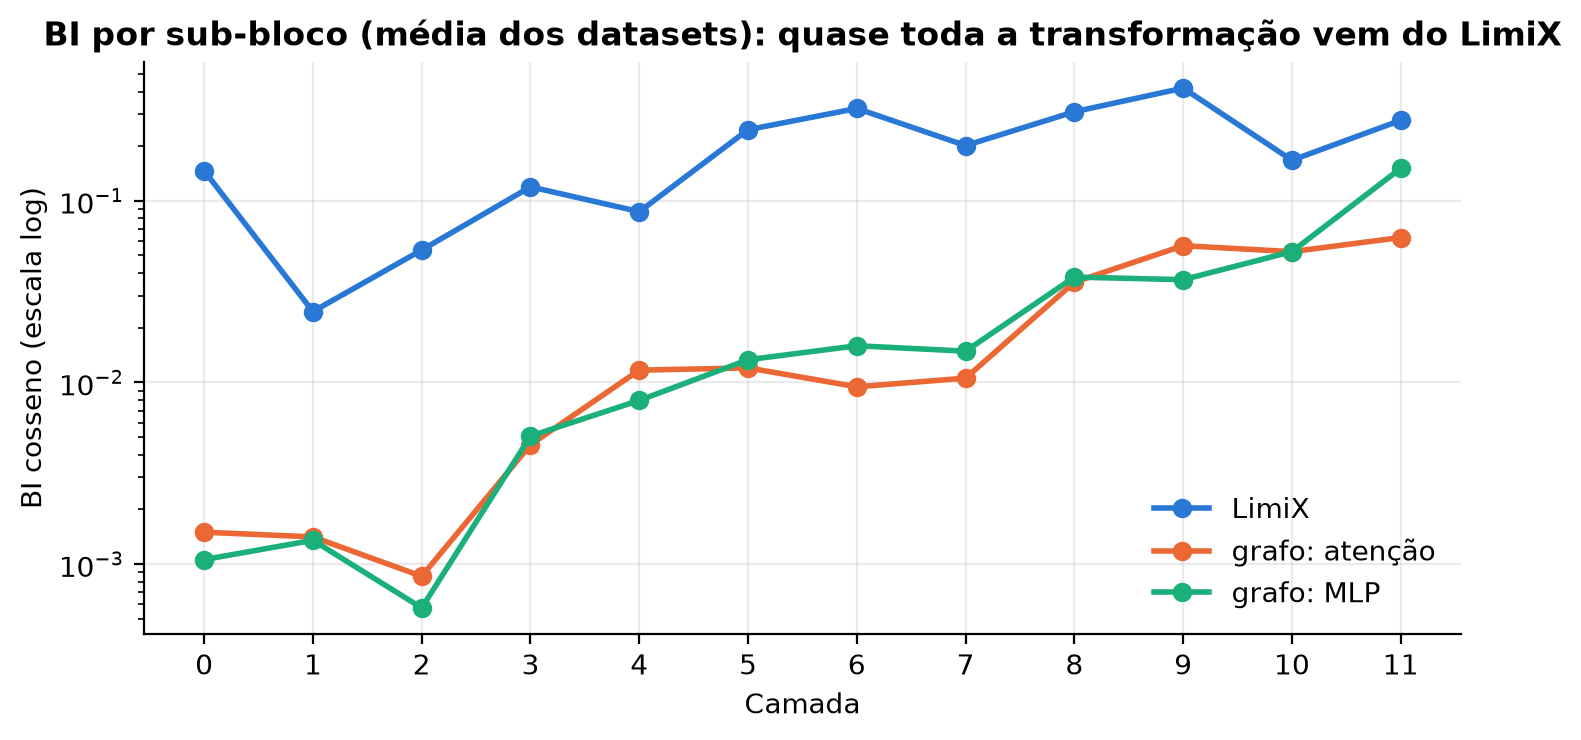
\includegraphics[width=\textwidth]{bi_por_subbloco.png}
\caption{BI por sub-bloco (LimiX, atenção de grafo, MLP de grafo).}
\label{fig:subbloco}
\end{figure}

\subsection{V4: ablação individual e importância real}

Cada camada foi removida sozinha, nas 3 sementes. A queda de desempenho é a importância real da camada.

\begin{table}[H]
\centering
\caption{Desempenho retido no teste (\%) ao remover \emph{uma única} camada. Em vermelho, quedas abaixo de 50\%.}
\label{tab:loo}
\setlength{\tabcolsep}{4pt}
\small
\begin{tabular}{@{}l*{12}{r}@{}}
\toprule
Dataset & L0 & L1 & L2 & L3 & L4 & L5 & L6 & L7 & L8 & L9 & L10 & L11 \\
\midrule
tolokers-2   & \ruim{$-3$}  & 59 & 95 & 96 & 83 & 96 & 91 & 92 & 77 & 90 & 98 & 98 \\
cora         & \ruim{0}     & 78 & 85 & 68 & 93 & 83 & \ruim{39} & \ruim{37} & \ruim{$-30$} & \ruim{$-11$} & 52 & \ruim{44} \\
pubmed       & \ruim{$-3$}  & \ruim{7} & 84 & 95 & 88 & 92 & 80 & 57 & \ruim{40} & \ruim{40} & 92 & 86 \\
city-roads-M & \ruim{$-40$} & 94 & 94 & 94 & 95 & 87 & 94 & 87 & 66 & 73 & 94 & 51 \\
artnet-views & \ruim{$-41$} & 96 & 93 & 96 & 93 & 95 & 89 & 93 & 67 & 67 & 93 & 71 \\
\bottomrule
\end{tabular}
\end{table}

\begin{itemize}
  \item \textbf{A camada 0 é indispensável}: removê-la sozinha leva todos os datasets ao nível do acaso ou abaixo ($-41\%$ a 0\%).
  \item \textbf{A camada 1 é crítica na classificação e dispensável na regressão}: retém 7\% no pubmed e 59\% no tolokers-2, mas 94--96\% nos datasets de regressão. O BI do token-alvo antecipa essa diferença; o BI de todos os tokens não.
  \item \textbf{Nenhuma camada é ``livre'' em todos os datasets.} As camadas 8 e 9 são importantes no cora e no pubmed, mas não no tolokers-2.
\end{itemize}

\begin{table}[H]
\centering
\caption{Correlação de Spearman ($\rho$) entre o BI de cada camada e sua importância real ($100 -$ retido na validação, ao remover a camada sozinha). $\rho$ positivo indica que BI alto corresponde a camada importante, que é o que o critério pressupõe.}
\label{tab:corr}
\begin{tabular}{@{}lcc@{}}
\toprule
Dataset & $\rho$ (BI de todos os tokens) & $\rho$ (BI do token-alvo) \\
\midrule
tolokers-2   & \ruim{$-0{,}27$} & 0,55 \\
cora         & 0,64  & 0,46 \\
pubmed       & 0,01  & 0,71 \\
city-roads-M & 0,62  & 0,82 \\
artnet-views & 0,66  & 0,75 \\
\midrule
Média        & 0,33  & \bom{0,66} \\
\bottomrule
\end{tabular}
\end{table}

\begin{figure}[H]
\centering
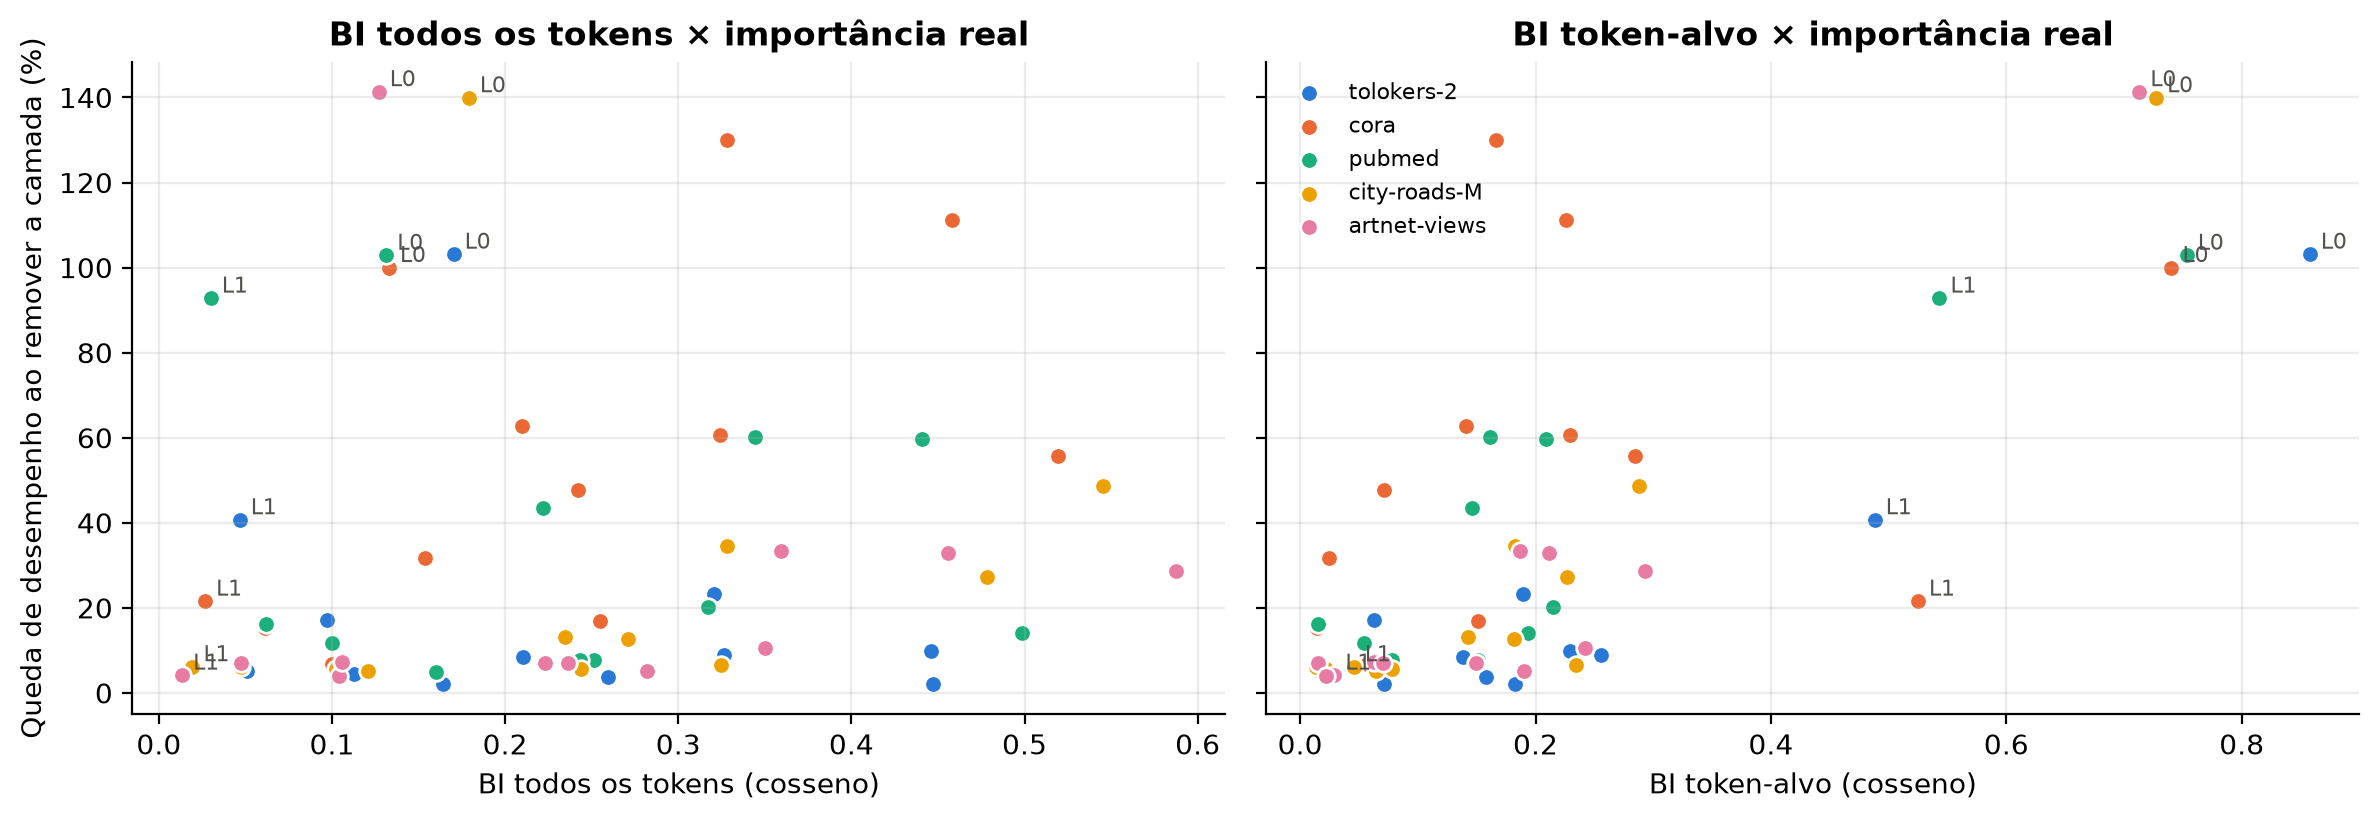
\includegraphics[width=\textwidth]{bi_vs_importancia.png}
\caption{BI $\times$ queda de desempenho ao remover a camada sozinha. As camadas 0 e 1 estão anotadas.}
\label{fig:bivsimp}
\end{figure}

\textbf{V4 é atendido apenas em parte.} A correlação é fraca com o BI de todos os tokens (0,33 em média, e negativa no tolokers-2) e moderada com o BI do token-alvo (0,66).

\subsection{V2 e V3: curvas de poda}

\begin{table}[H]
\centering
\caption{Camadas removidas em cada estratégia, para $k = 1, \dots, 5$ (a poda é cumulativa).}
\label{tab:ordens}
\small
\begin{tabular}{@{}llll@{}}
\toprule
Estratégia & Dataset & Ordem de remoção (primeiras 5) & Camadas removidas com $k=5$ \\
\midrule
\multirow{3}{*}{BI de todos os tokens}
 & tolokers-2 & 1, 2, 4, 3, 10 & \{1, 2, 3, 4, 10\} \\
 & cora, pubmed & 1, 2, 4, 0, 3 & \{\ruim{0}, 1, 2, 3, 4\} \\
 & city-roads-M, artnet-views & 1, 2, 3, 4, 0 & \{\ruim{0}, 1, 2, 3, 4\} \\
\midrule
\multirow{2}{*}{BI do token-alvo}
 & tolokers-2, cora, pubmed & 2, 3, 4, 10, 7 & \{2, 3, 4, 7, 10\} \\
 & city-roads-M, artnet-views & 2, 3, 1, 4, 10 & \{1, 2, 3, 4, 10\} \\
\midrule
\multirow{5}{*}{Ablação individual (val)}
 & tolokers-2 & 11, 10, 5, 3, 2 & \{2, 3, 5, 10, 11\} \\
 & cora & 4, 2, 1, 5, 3 & \{1, 2, 3, 4, 5\} \\
 & pubmed & 5, 4, 10, 3, 2 & \{2, 3, 4, 5, 10\} \\
 & city-roads-M & 4, 3, 10, 1, 2 & \{1, 2, 3, 4, 10\} \\
 & artnet-views & 1, 3, 5, 2, 7 & \{1, 2, 3, 5, 7\} \\
\bottomrule
\end{tabular}
\end{table}

\begin{table}[H]
\centering
\caption{Desempenho retido no teste (\%) em função do número de camadas removidas $k$ (média de 3 sementes; a linha ``Aleatória'' é a mediana das 5 ordens aleatórias). Em negrito, valores $\geq 95\%$; em vermelho, valores $\leq 0\%$ (nível do acaso ou pior).}
\label{tab:curvas}
\small
\begin{tabular}{@{}llrrrrrr@{}}
\toprule
Dataset & Estratégia & $k=1$ & $k=2$ & $k=3$ & $k=4$ & $k=5$ & $k=6$ \\
\midrule
\multirow{4}{*}{tolokers-2}
 & BI todos os tokens & 59,3 & 79,5 & 64,3 & 75,2 & 44,1 & 27,2 \\
 & BI token-alvo      & 94,8 & 91,0 & 84,5 & 62,4 & 59,2 & 21,0 \\
 & Ablação (val)      & \bom{97,9} & 92,3 & 83,5 & 52,1 & 26,6 & 4,7 \\
 & Aleatória          & 90,4 & 78,7 & 53,0 & 30,3 & 21,3 & 24,3 \\
\midrule
\multirow{4}{*}{cora}
 & BI todos os tokens & 78,4 & 74,2 & 43,2 & \ruim{$-68{,}1$} & \ruim{$-48{,}2$} & \ruim{$-53{,}2$} \\
 & BI token-alvo      & 84,8 & 94,5 & 62,8 & \ruim{$-18{,}0$} & \ruim{$-56{,}8$} & \ruim{$-52{,}4$} \\
 & Ablação (val)      & 93,2 & 64,4 & 43,2 & \ruim{$-56{,}5$} & \ruim{$-49{,}1$} & \ruim{$-49{,}3$} \\
 & Aleatória          & 55,1 & \ruim{$-11{,}0$} & \ruim{$-37{,}6$} & \ruim{$-64{,}4$} & \ruim{$-53{,}4$} & \ruim{$-53{,}4$} \\
\midrule
\multirow{4}{*}{pubmed}
 & BI todos os tokens & 7,2 & 71,0 & 71,8 & \ruim{0,0} & \ruim{$-2{,}3$} & \ruim{$-77{,}5$} \\
 & BI token-alvo      & 83,9 & 90,6 & 58,4 & 50,3 & 10,1 & \ruim{$-2{,}8$} \\
 & Ablação (val)      & 92,3 & 39,8 & 55,9 & \ruim{$-1{,}3$} & 0,1 & \ruim{$-11{,}2$} \\
 & Aleatória          & 56,0 & 20,7 & \ruim{$-10{,}7$} & \ruim{$-4{,}7$} & \ruim{$-75{,}0$} & \ruim{0,0} \\
\midrule
\multirow{4}{*}{city-roads-M}
 & BI todos os tokens & 93,9 & 90,3 & 86,9 & 78,2 & \ruim{$-56{,}5$} & \ruim{$-28{,}1$} \\
 & BI token-alvo      & 93,9 & 91,0 & 86,9 & 78,2 & 72,7 & 53,4 \\
 & Ablação (val)      & 95,0 & 88,4 & 80,3 & 73,2 & 72,7 & 27,9 \\
 & Aleatória          & 93,9 & 77,0 & 58,1 & 10,5 & 4,0 & \ruim{$-0{,}9$} \\
\midrule
\multirow{4}{*}{artnet-views}
 & BI todos os tokens & \bom{95,8} & 82,6 & 84,8 & 63,1 & \ruim{$-59{,}7$} & \ruim{$-37{,}1$} \\
 & BI token-alvo      & 93,1 & 86,7 & 84,8 & 63,1 & 52,7 & 33,1 \\
 & Ablação (val)      & \bom{95,8} & 90,9 & 76,1 & 62,3 & 24,3 & 24,3 \\
 & Aleatória          & 92,8 & 68,7 & 57,5 & 16,7 & \ruim{$-1{,}5$} & \ruim{$-5{,}1$} \\
\bottomrule
\end{tabular}
\end{table}

\begin{figure}[H]
\centering
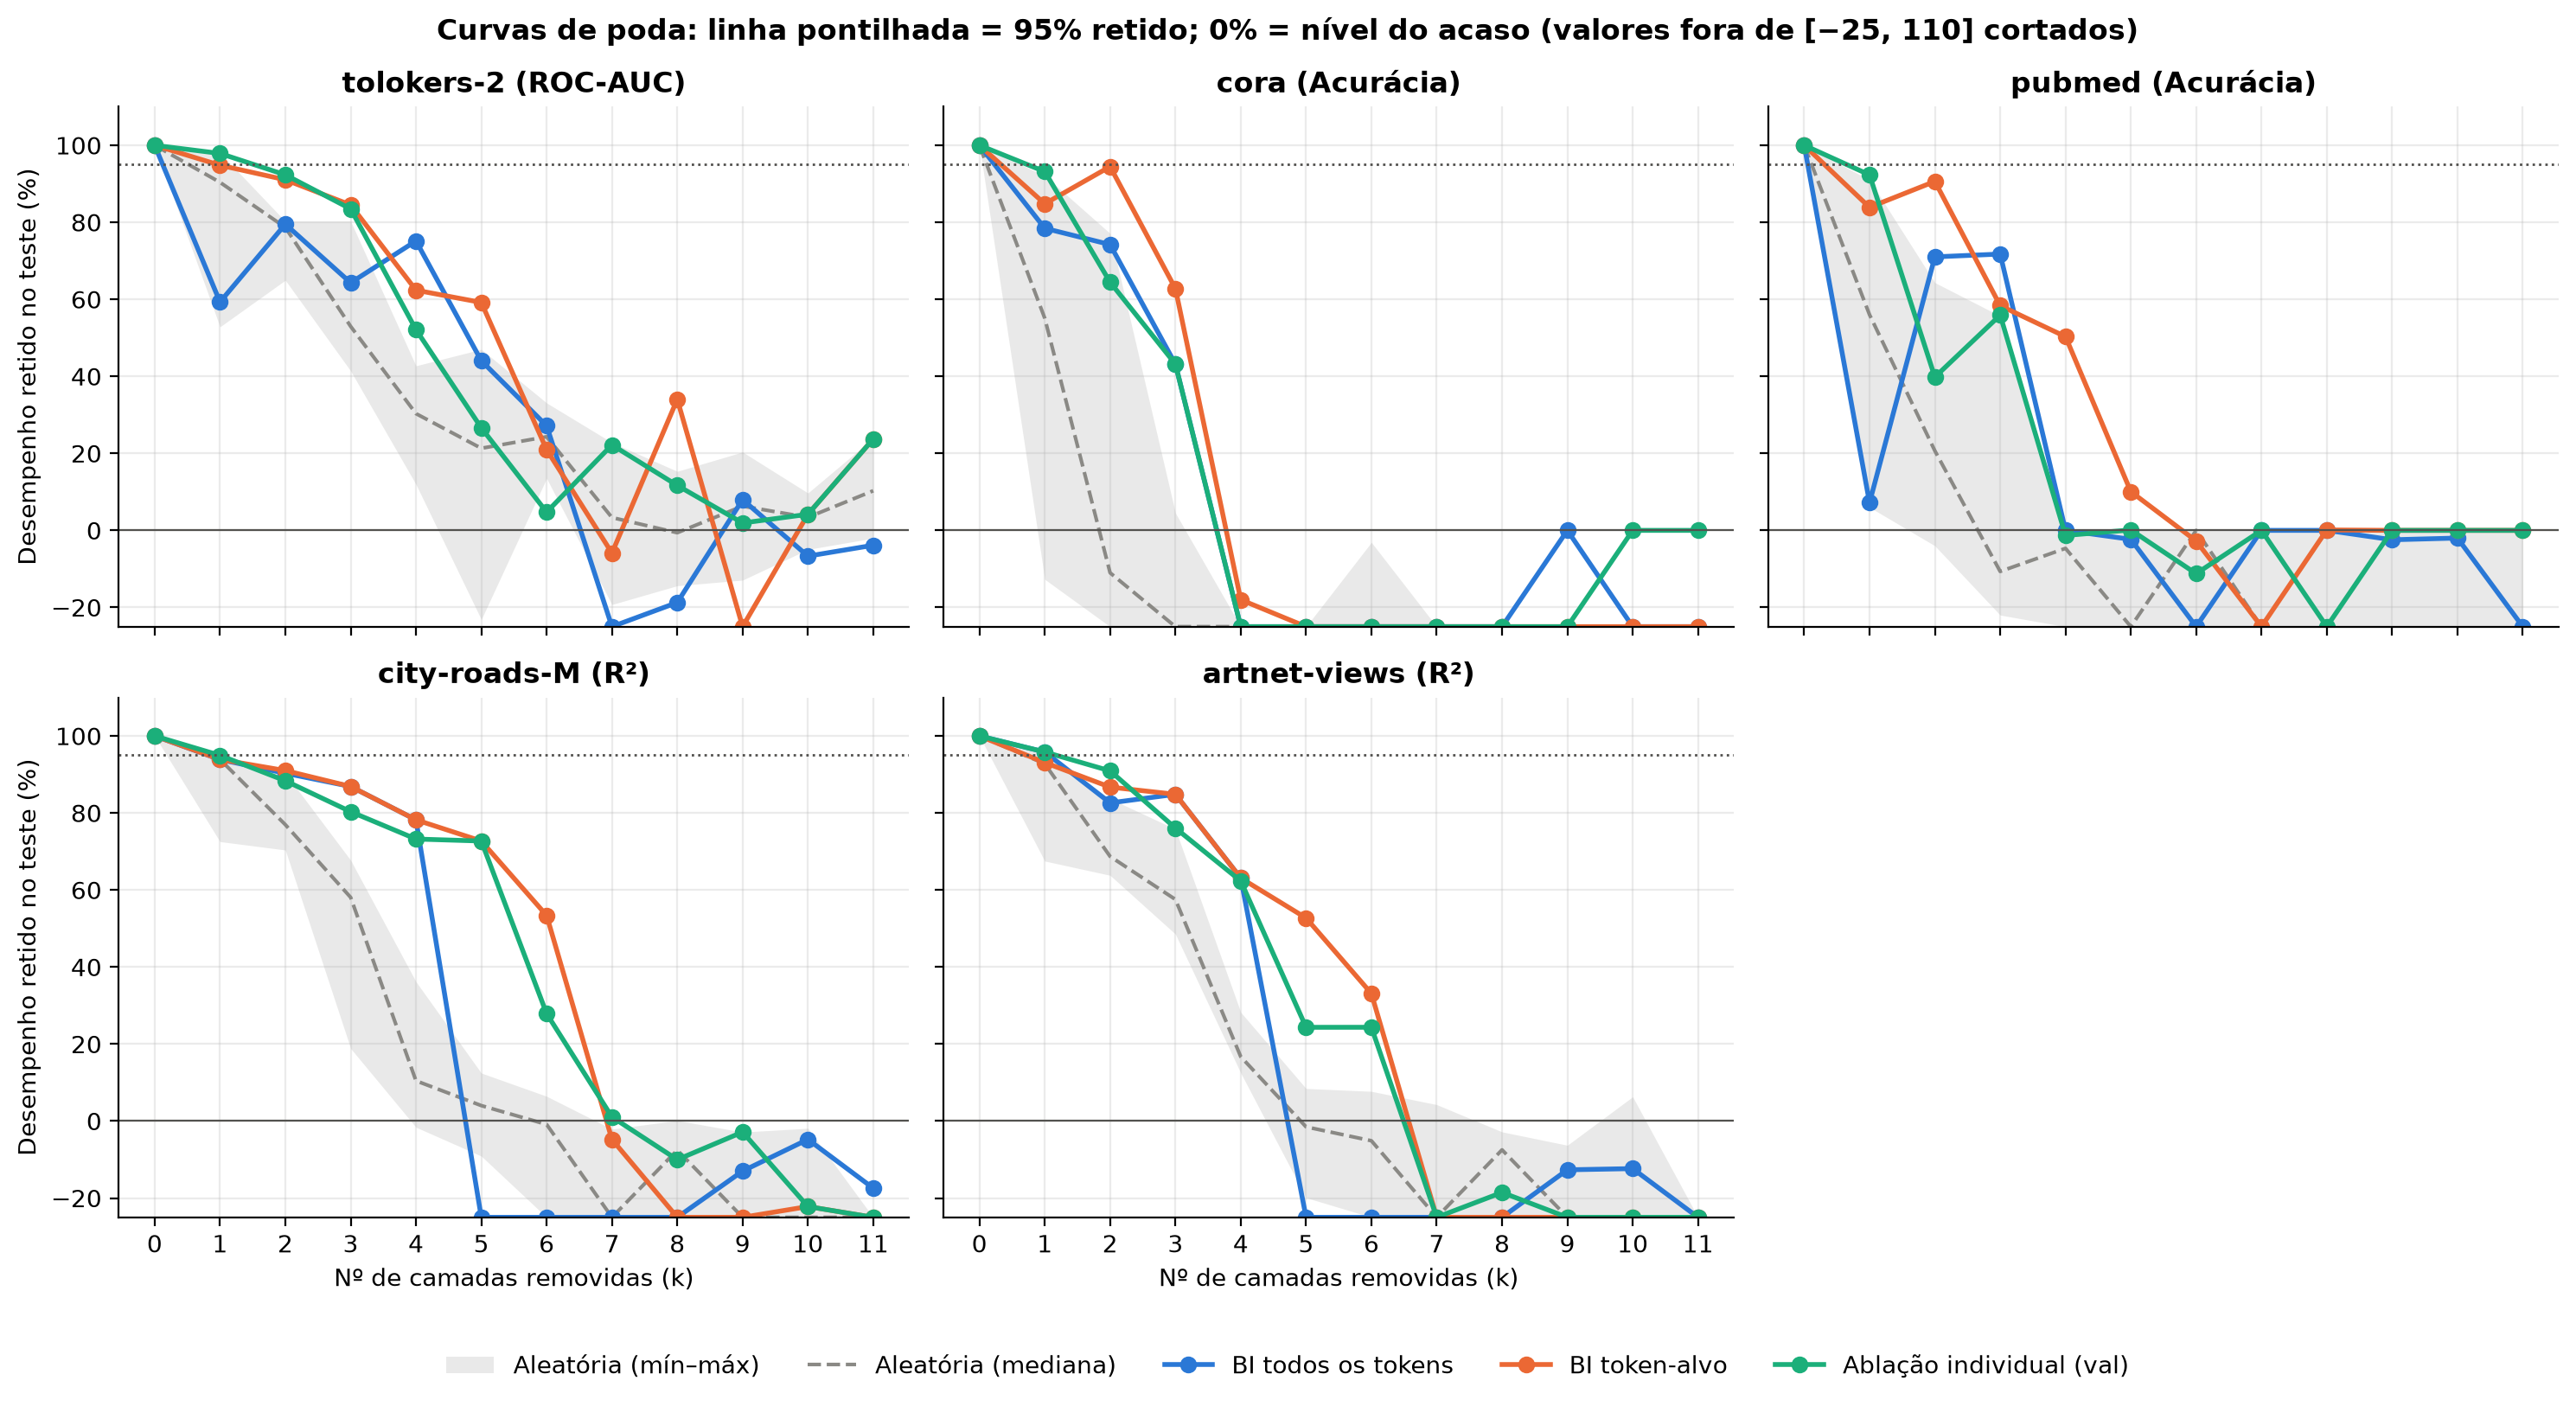
\includegraphics[width=\textwidth]{curvas_poda.png}
\caption{Curvas de poda. Linha pontilhada: 95\% retido. Faixa cinza: mínimo e máximo das 5 ordens aleatórias.}
\label{fig:curvas}
\end{figure}

\begin{table}[H]
\centering
\caption{Desempenho retido médio nos 5 datasets ao remover 3 camadas.}
\label{tab:k3}
\begin{tabular}{@{}lr@{}}
\toprule
Estratégia & Retido com $k=3$ \\
\midrule
BI do token-alvo         & \bom{75,5\%} \\
BI de todos os tokens    & 70,2\% \\
Ablação individual (val) & 67,8\% \\
Aleatória (mediana)      & 24,1\% \\
\bottomrule
\end{tabular}
\end{table}

\begin{itemize}
  \item \textbf{V3 é atendido.} Com $k=3$, o BI de todos os tokens vence a ordem aleatória nos 5 datasets (70\% contra 24\% retido, em média). O BI do token-alvo é ainda melhor (75,5\%).
  \item \textbf{V2 não é atendido além de uma camada.} O limite de 95\% só é alcançado com $k=1$ e só em dois datasets: artnet-views (BI de todos os tokens e ablação) e tolokers-2 (ablação). Nos demais, o melhor resultado com $k=1$ fica entre 92\% e 95\%. Com 2 ou 3 camadas removidas, a perda já fica entre 10\% e 50\%.
  \item \textbf{O BI de todos os tokens falha justamente onde remove as camadas 0 e 1.} No pubmed, com $k=1$, ele remove a camada 1 e o desempenho retido cai para 7\%. Com $k=5$, a camada 0 entra na lista e city-roads-M e artnet-views, que vinham estáveis (78\% e 63\% com $k=4$), despencam para $-57\%$ e $-60\%$. O BI do token-alvo, que nunca remove a camada 0 nas primeiras posições, mantém 73\% e 53\% nesses mesmos pontos.
  \item \textbf{Nem a ablação passa no critério}, embora escolha as camadas olhando rótulos de validação. Isso mostra que o limite não vem de uma falha do BI: as camadas do GraphPFN não são redundantes.
  \item \textbf{As curvas têm ruído entre valores vizinhos de $k$}: por exemplo, no cora o BI do token-alvo retém 84,8\% com $k=1$ e 94,5\% com $k=2$. A tendência geral é clara, mas diferenças de poucos pontos entre $k$ vizinhos não devem ser interpretadas.
\end{itemize}

\subsection{Custo}

\begin{table}[H]
\centering
\caption{Parâmetros e latência em função do número de camadas removidas. Latência medida no city-roads-M (57\,073 nós), mediana de 3 execuções, incluindo pré e pós-processamento.}
\label{tab:custo}
\begin{tabular}{@{}rrrrrr@{}}
\toprule
$k$ & Camadas & Parâmetros (M) & Redução & Latência (s) & Redução \\
\midrule
0  & 12 & 20,09 & --     & 3,97 & --     \\
2  & 10 & 16,84 & 16,2\% & 3,36 & 15,3\% \\
4  & 8  & 13,59 & 32,3\% & 2,66 & 33,0\% \\
6  & 6  & 10,35 & 48,5\% & 2,07 & 47,8\% \\
8  & 4  & 7,10  & 64,7\% & 1,46 & 63,2\% \\
10 & 2  & 3,85  & 80,8\% & 0,81 & 79,7\% \\
\bottomrule
\end{tabular}
\end{table}

O ganho de custo é linear: cada camada vale cerca de 8\% dos parâmetros e 8\% da latência. A perda de desempenho cresce muito mais rápido que isso.

%==============================================================================
\section{Comparação com a avaliação anterior}
%==============================================================================

Uma avaliação anterior, com limiares fixos de BI (Tier 1: $BI \leq 0{,}15$, removendo as camadas $\{0,1,2,3,4\}$; Tier 2: $BI \leq 0{,}20$, removendo $\{0,1,2,3,4,7\}$), sugeria que a poda não causava perda. A diferença não está no BI, que deu valores semelhantes, e sim na avaliação:

\begin{enumerate}
  \item \textbf{O modelo completo estava no nível do acaso.} Nos datasets do AnyGraph, o baseline tinha ROC-AUC de 0,44 a 0,52 (acurácia de 0,13 no cora). Com o baseline já chutando, modelo podado e completo ``empatavam''.
  \item \textbf{O grafo quase não tinha arestas.} Eram sorteados 500 nós e usado o subgrafo induzido; no cora isso deu 676 arestas, das quais 500 eram self-loops adicionados manualmente. O pipeline oficial faz o oposto: remove self-loops e simetriza o grafo.
  \item \textbf{O pré-processamento não era o oficial}: PCA de 32 dimensões direto, sem \texttt{prepare\_features\_tensor}, e alvo de regressão sem padronização. Os splits eram aleatórios, com uma semente e 200 nós de teste.
  \item \textbf{Acurácia e F1 não detectavam a queda.} Na classificação binária, com limiar fixo de 0,5, o modelo previa sempre a classe majoritária, e acurácia e F1 ficavam idênticos com e sem poda. O ROC-AUC, no entanto, já caía para o nível do acaso (por exemplo, city-reviews: de 0,90 para 0,53), e o $R^2$ médio da regressão caía de 0,14 para $-0{,}34$.
  \item \textbf{Os limiares incluíam a camada 0}, que tem BI 0,148 na média de todos os tokens, mas é a única camada indispensável. O arredondamento para 2 casas também incluiu a camada 3 (0,153) no Tier 1.
  \item \textbf{O BI de referência incluía um grafo sintético} (features gaussianas e rótulos aleatórios) na média entre datasets.
\end{enumerate}

Nos casos em que o baseline antigo funcionava (ROC-AUC binário e $R^2$), ele já mostrava o mesmo que este relatório: remover 5 ou 6 camadas leva o modelo ao nível do acaso.

%==============================================================================
\section{Conclusões}
%==============================================================================

\begin{table}[H]
\centering
\caption{Veredito.}
\label{tab:veredito}
\begin{tabular}{@{}lp{9.5cm}@{}}
\toprule
Critério & Resultado \\
\midrule
V1 Baseline válido & \textbf{Sim.} Modelo completo bem acima do acaso em todos os datasets. \\
V2 Poda retém $\geq 95\%$ & \textbf{Não.} No máximo 1 camada ($\approx 8\%$ dos parâmetros), e só em 2 de 5 datasets. \\
V3 BI melhor que aleatório & \textbf{Sim.} 70\% contra 24\% retido com $k=3$; vence em 5 de 5 datasets. \\
V4 BI reflete importância real & \textbf{Em parte.} $\rho = 0{,}33$ (todos os tokens) e $0{,}66$ (token-alvo). \\
\bottomrule
\end{tabular}
\end{table}

\textbf{Remover camadas inteiras do GraphPFN escolhidas por Block Influence, sem re-treino, não é uma poda válida além de uma camada.} Ao contrário dos LLMs, em que o ShortGPT encontra camadas quase redundantes, as 12 camadas do LimiX-16M são todas usadas.

\begin{itemize}
  \item O BI ajuda a ordenar as camadas (é muito melhor que o acaso), mas a ordem não basta: mesmo a ordem quase ótima, escolhida por ablação com rótulos de validação, perde mais de 5\% a partir de 2 camadas.
  \item O BI calculado como média sobre todos os tokens é enganoso neste modelo, porque os tokens de feature dominam a média e escondem que as camadas 0 e 1 são as que mais alteram o token-alvo. Para modelos que decodificam apenas parte dos tokens, o BI deve ser medido nesses tokens.
  \item Os adaptadores de grafo alteram muito pouco o estado (BI até 0,09, exceto o MLP de grafo da camada 11) e representam 18\% dos parâmetros de cada camada.
\end{itemize}

\subsection*{Possíveis próximos passos}

\begin{enumerate}
  \item Usar o BI do token-alvo como critério padrão e nunca remover as camadas 0 e 1 na classificação.
  \item Testar poda seguida de um ajuste curto (\emph{healing}), como é feito em LLMs, para recuperar o desempenho com 2 a 4 camadas removidas.
  \item Testar poda de granularidade menor: remover sub-blocos (por exemplo, os adaptadores de grafo de baixo BI ou um dos MLPs do bloco LimiX) em vez da camada inteira. Este caso não foi avaliado aqui.
\end{enumerate}

\vspace{1em}
\noindent\small\textit{Reprodutibilidade}: todos os números vêm de \texttt{GraphFPN/analise\_camadas\_e\_poda\_graphpfn.ipynb} e dos arquivos CSV em \texttt{Block\_Influence\_results/graphfpn\_analise\_unificada/} (\texttt{baseline.csv}, \texttt{block\_influence.csv}, \texttt{ablacao\_individual.csv}, \texttt{curvas\_poda.csv}, \texttt{custo\_poda.csv}, \texttt{veredito.csv}).

\end{document}
